\documentclass[11pt]{article}

\usepackage[utf8]{inputenc}
\usepackage[french]{babel}
% ============================================================
% SHARED PREAMBLE -- included by Internship_Report_EN.tex and
% Rapport_de_Stage_FR.tex. Keeps both language versions visually
% identical. Edit style here, not in the two content files.
% ============================================================

\usepackage[T1]{fontenc}
\usepackage[margin=1in]{geometry}
\usepackage{graphicx}
\graphicspath{{../plots/}{./figures/}}

\usepackage{amsmath}
\usepackage{amssymb}

\usepackage{booktabs}
\usepackage{array}
\usepackage{tabularx}
\usepackage{adjustbox}
\usepackage{caption}
\usepackage[table]{xcolor}
\usepackage{enumitem}

\usepackage{tikz}
\usetikzlibrary{arrows.meta, positioning}

\usepackage{fancyhdr}
\usepackage{titlesec}

% ------------------------------------------------------------
% COLOR
% ------------------------------------------------------------
\definecolor{umorange}{RGB}{215,74,42}

% ------------------------------------------------------------
% TABLE DEFAULTS
% ------------------------------------------------------------
\AtBeginEnvironment{table}{\centering}
\captionsetup[table]{justification=centering, singlelinecheck=false}
\captionsetup[figure]{justification=centering, singlelinecheck=false}
\renewcommand{\arraystretch}{1.2}
\newcolumntype{Y}{>{\centering\arraybackslash}X}

% Light rule usable inside tabular/tabularx bodies between rows
\newcommand{\rowrule}{\midrule[0.2pt]}

% ------------------------------------------------------------
% HEADER / FOOTER
% ------------------------------------------------------------
\newcommand{\ReportHeaderLeft}{}
\newcommand{\ReportHeaderRight}{}

\pagestyle{fancy}
\fancyhf{}
\renewcommand{\headrulewidth}{0.4pt}
\renewcommand{\footrulewidth}{0pt}
\fancyhead[L]{\slshape\small\ReportHeaderLeft}
\fancyhead[R]{\slshape\small\ReportHeaderRight}
\fancyfoot[C]{\thepage}

\fancypagestyle{plain}{
  \fancyhf{}
  \fancyfoot[C]{\thepage}
  \renewcommand{\headrulewidth}{0pt}
  \renewcommand{\footrulewidth}{0pt}
}

% ------------------------------------------------------------
% SECTION / SUBSECTION STYLE -- bold title + thin orange rule
% ------------------------------------------------------------
\titleformat{\section}
  {\Large\bfseries}
  {\thesection}
  {0.6em}
  {}
  [{\color{umorange}\titlerule[1pt]}]
\titlespacing*{\section}{0pt}{3.2ex plus 1ex minus .2ex}{1.6ex plus .2ex}

\titleformat{\subsection}
  {\large\bfseries}
  {\thesubsection}
  {0.6em}
  {}
\titlespacing*{\subsection}{0pt}{2.6ex plus 1ex minus .2ex}{1ex plus .2ex}

\titleformat{\subsubsection}
  {\bfseries}
  {\thesubsubsection}
  {0.6em}
  {}
\titlespacing*{\subsubsection}{0pt}{2ex plus 1ex minus .2ex}{0.8ex plus .2ex}

% ------------------------------------------------------------
% TIKZ NODE STYLE -- shared by every pipeline/workflow diagram
% ------------------------------------------------------------
\tikzset{
  rbox/.style={draw, rounded corners, fill=umorange!12, align=center,
               minimum height=1.05cm, text width=#1, font=\small},
  rbox/.default=2.6cm,
  flow/.style={-{Latex[length=2.2mm]}, thick}
}


\newcommand{\ReportTitleShort}{Rapport de stage -- Schémas de capture de choc augmentés par IA}
\renewcommand{\ReportHeaderLeft}{\ReportTitleShort}
\renewcommand{\ReportHeaderRight}{Yasser Baouzil}

\begin{document}

% ============================================================
% PAGE DE TITRE
% ============================================================
\begin{titlepage}
\thispagestyle{empty}

\begin{center}

\includegraphics[width=0.55\textwidth]{um6p_college_of_computing_logo.png}
\end{center}

\vspace{4.5cm}

\begin{center}
{\Huge\bfseries Rapport de stage}\\[1.2cm]
{\Large Schémas de capture de choc augmentés par apprentissage\\
automatique pour les lois de conservation~: de l'apprentissage\\
par imitation à une fonction de perte physique déroulée}\\[0.4cm]
{\large UM6P -- College of Computing}
\end{center}

\vspace{3cm}

\begin{center}
\begin{tabular}{ll}
\textbf{Étudiant} & Yasser Baouzil \\
\textbf{Établissement d'accueil} & UM6P -- College of Computing \\
\textbf{Tuteur de stage} & Radouan Boukharfane \\
\textbf{Encadrant académique} & Radouan Boukharfane \\
\textbf{Période} & Du 01/06/2026 au 01/08/2026 \\
\textbf{Durée} & 2 mois \\
\textbf{Niveau} & 1\up{ère} année du cycle ingénieur \\
\end{tabular}
\end{center}

\vfill

\begin{center}
\color{umorange}\rule{0.5\textwidth}{0.6pt}
\end{center}

\begin{center}
Année universitaire 2025-2026
\end{center}

\end{titlepage}

% ============================================================
% SOMMAIRE
% ============================================================
\tableofcontents
\thispagestyle{plain}
\newpage

% ============================================================
\section{Résumé}

Ce rapport présente le travail réalisé durant un stage de deux mois à
l'UM6P -- College of Computing, sous la supervision de Radouan Boukharfane.
Le projet étudie si un réseau de neurones peut améliorer des schémas
classiques de capture de choc en volumes finis (WENO5, TENO5) pour les
lois de conservation hyperboliques, et surtout si la manière dont ce
réseau est \emph{entraîné} détermine le type d'amélioration réellement
atteignable.

Le travail se construit en deux couches. La première reproduit et étend un
résultat existant de la littérature~: un réseau entraîné par
\emph{imitation} pour reproduire la décision de reconstruction d'un schéma
classique, évalué contre ce même schéma sur l'advection scalaire,
l'équation de Burgers, et le système d'Euler (tube à choc de Sod,
problème de Shu--Osher). Par construction, un réseau entraîné par
imitation ne peut pas dépasser systématiquement la qualité du schéma
qu'il imite -- les mesures le confirment directement.

La seconde couche, plus importante, teste une alternative proposée par
l'encadrant de stage~: une \emph{fonction de perte physique déroulée}
(Unrolled Physics Loss). Plutôt que d'imiter la décision d'un schéma
classique stencil par stencil, le réseau est entraîné en le faisant
tourner sur plusieurs pas de simulation réels, puis en jugeant la
trajectoire obtenue par rapport à la solution réelle. Cela a nécessité une
réécriture complète, entièrement différentiable, en JAX du c\oe{}ur numérique
du projet, puisque rien dans le code NumPy/Keras d'origine n'est
différentiable de bout en bout.

Cette nouvelle approche produit les seules victoires réelles et vérifiées
du projet contre le schéma classique~: sur les benchmarks scalaires
Burgers et advection, et sur le problème d'Euler Shu--Osher. Elle révèle
aussi un véritable mode de défaillance numérique, diagnostiqué avec
précision (un problème de conditionnement de la base propre de Roe sous
une reconstruction neuronale évolutive), ainsi qu'un plafond structurel
réel sur le tube à choc de Sod qu'aucun réglage supplémentaire ne permet de
dépasser. Les résultats positifs comme négatifs sont rapportés avec le
même niveau de détail, car la valeur de ce stage réside dans la
compréhension du \emph{pourquoi} de chaque résultat, pas seulement dans
les chiffres finaux.

% ============================================================
\section{Introduction}

Les schémas de capture de choc tels que WENO (Weighted Essentially
Non-Oscillatory) et TENO (Targeted Essentially Non-Oscillatory)
constituent le socle numérique des simulations haute-fidélité
d'écoulements compressibles. Ils reconstruisent un interpolant lisse et
d'ordre élevé partout, sauf au voisinage d'une discontinuité, où ils
basculent vers un schéma d'ordre plus faible mais non oscillant. La règle
qui décide \emph{où} basculer est elle-même conçue à la main~: un
indicateur de régularité, comparé à un seuil, calculé indépendamment à
chaque interface de cellule.

Remplacer cette règle par un réseau de neurones entraîné est une idée
séduisante~: un réseau peut en principe apprendre une frontière de
décision plus finement ajustée aux données qu'une formule analytique fixe.
Le résultat publié WENO5-NN (Stevens \& Colonius, 2020) montre que cela
est possible pour un schéma WENO5. Ce stage reproduit d'abord ce résultat,
puis pose une question plus difficile~: la même idée peut-elle être
poussée plus loin pour TENO5 -- et, plus fondamentalement, la façon dont le
réseau est entraîné change-t-elle la nature même de l'amélioration
possible~?

Le rapport est organisé dans l'ordre où la question a réellement été
étudiée~: contexte numérique, approche par imitation d'origine et son
plafond structurel, la fonction de perte physique déroulée proposée comme
alternative, l'infrastructure différentiable qu'elle a nécessitée, et les
résultats et modes de défaillance obtenus sur les problèmes scalaires et
sur le système (Euler).

% ============================================================
\section{Contexte du stage}

Le stage s'est déroulé à l'UM6P -- College of Computing, sur deux mois
(juin--août 2026), sous la supervision de Radouan Boukharfane, qui a
également proposé la question de recherche centrale du stage ainsi que sa
seconde phase (la fonction de perte physique déroulée). Le sujet, tel
qu'indiqué sur la fiche technique du stage, était \emph{« Machine
learning-based numerical scheme for CFD »}, avec trois missions
énoncées~: une revue de littérature, la construction d'un réseau de
neurones calculant les fonctions de pondération utilisées dans un schéma
de type WENO, et l'évaluation de ses performances.

Le stage s'appuie directement sur un code source existant, en accès
libre, implémentant l'article WENO5-NN d'origine. Plutôt que de repartir
de zéro, le travail étend ce code à TENO5, en reproduit d'abord les
résultats publiés comme référence, puis teste une méthodologie
d'entraînement absente des travaux publiés.

Le sujet étant une question de recherche plutôt qu'un cahier des charges
figé, le travail a été organisé comme une séquence d'expériences
falsifiables plutôt que comme un plan d'implémentation linéaire~: chaque
phase propose un mécanisme précis, le teste contre la solution réelle, et
le conserve, le corrige ou l'abandonne selon le résultat mesuré. Cette
discipline expérimentale se retrouve directement dans les résultats
présentés plus loin dans ce document.

% ============================================================
\section{Objectifs, périmètre et missions du projet}

L'objectif du stage était de déterminer si un réseau de neurones peut
améliorer TENO5, un schéma classique de capture de choc à l'état de
l'art, et de le faire avec des résultats mesurés par rapport à la solution
réelle, et non par rapport à la seule sortie du schéma classique.

Les trois missions définies en début de stage étaient~:

\begin{itemize}
    \item \textbf{Bibliographie}~: étudier la littérature sur les schémas
    WENO/TENO augmentés par apprentissage automatique, ainsi que le
    principe de Boundary Variation Diminishing (BVD) utilisé plus tard
    dans la fonction de perte.
    \item \textbf{Réseau de neurones}~: construire un réseau calculant la
    fonction de pondération/sélection à l'intérieur d'une reconstruction
    de type WENO (quel candidat garder à chaque interface).
    \item \textbf{Évaluation des performances}~: mesurer la précision de
    ce réseau par rapport au schéma classique qu'il augmente, sur des
    problèmes de test canoniques, pas seulement sur des données
    d'entraînement mises de côté.
\end{itemize}

Le périmètre a volontairement été limité aux schémas d'ordre cinq (WENO5,
TENO5) sur des problèmes de test scalaires et Euler en une dimension~:
advection linéaire, équation de Burgers, tube à choc de Sod, et problème
de Shu--Osher. Les ordres supérieurs (WENO3/WENO7, TENO3/TENO7) et les
problèmes multidimensionnels existent comme modules de reconstruction dans
le code, mais ont été explicitement exclus du périmètre d'entraînement,
puisqu'aucun jeu de données d'entraînement d'ordre 3 ou 7 n'existe et que
sa construction ne faisait pas partie des missions énoncées.

Un quatrième objectif, non planifié, est apparu directement des deux
premiers mois de travail~: une fois établi que l'entraînement par
imitation possède un plafond structurel (section~\ref{sec:volet2}), le
périmètre du stage s'est élargi à la conception, l'implémentation et
l'évaluation d'un paradigme d'entraînement alternatif -- la fonction de
perte physique déroulée -- proposé par l'encadrant académique précisément
pour lever ce plafond.

% ============================================================
\section{Méthodologie de travail}

Le projet a été organisé comme une séquence chronologique d'expériences
numérotées (21 au total à la fin du stage), chacune avec un objectif
énoncé, un critère de falsification concret, et un résultat documenté --
qu'il soit positif, négatif ou partiel. Cette discipline a été adoptée
tôt, après qu'une première tentative (non instrumentée) a rendu difficile
de distinguer une amélioration réelle d'un artefact de mesure.

Deux critères d'évaluation ont été utilisés tout au long du projet,
appliqués de façon cohérente à chaque expérience~:

\begin{itemize}
    \item \texttt{beats\_teacher}~: l'erreur du réseau par rapport à la
    solution \emph{réelle} est strictement inférieure à celle du schéma
    classique par rapport à la même solution réelle. C'est le critère
    utilisé pour chaque victoire revendiquée dans ce rapport.
    \item \texttt{teacher\_fidelity}~: l'erreur du réseau reste dans une
    marge réduite (2\%) de celle du schéma classique. Ce critère, plus
    souple, n'a été utilisé que pour des tests d'acceptation précoces et
    n'est jamais utilisé pour revendiquer une supériorité.
\end{itemize}

Chaque expérience a été exécutée, mesurée selon les deux critères sur des
benchmarks canoniques (hors entraînement), et documentée immédiatement --
y compris les expériences qui ont dégradé les résultats. C'est pourquoi le
journal d'expériences interne du projet
(\texttt{Documentation/Results.md}) recense 21 phases plutôt qu'une
poignée de succès triés~: plusieurs correctifs qui semblaient corrects sur
le papier (section~\ref{sec:instabilite}) ont mesurablement échoué et ont
dû être annulés ou remplacés.

Un second choix méthodologique, adopté après la perte d'un point de
sauvegarde fonctionnel lors d'une expérience non sauvegardée, a été de
valider et sauvegarder immédiatement chaque résultat vérifié comme bon,
avant de démarrer l'expérience suivante par-dessus.

% ============================================================
\section{Contexte scientifique~: méthodes en volumes finis pour les lois de conservation}
\label{sec:fond-vf}

Une loi de conservation hyperbolique scalaire,
\[
\partial_t u + \partial_x f(u) = 0,
\]
et le système d'Euler compressible (sa généralisation vectorielle, où $u$
est le vecteur des variables conservées -- densité, quantité de mouvement,
énergie -- et $f(u)$ le flux physique correspondant) sont tous deux
résolus ici par la méthode des lignes~: le domaine spatial est divisé en
$N$ cellules, chaque cellule $i$ stocke une moyenne de cellule $u_i$, et
l'équation est avancée en estimant le flux à chaque interface $i+1/2$ puis
en intégrant
\[
\frac{d u_i}{dt} = -\frac{1}{\Delta x}\left(\hat f_{i+1/2} - \hat f_{i-1/2}\right)
\]
en temps avec un schéma de Runge--Kutta explicite. Dans tout le projet, il
s'agit du SSPRK3 d'ordre trois (la forme à préservation forte de la
stabilité de Shu \& Osher, utilisée de façon identique dans l'article de
Stevens \& Colonius), choisi car chacune de ses étapes est elle-même une
combinaison convexe de pas d'Euler explicite, si bien qu'il ne peut pas
amplifier un état déjà non oscillant~:
\begin{align*}
u^{(1)} &= u^{(n)} + \Delta t\, L(u^{(n)}), \\
u^{(2)} &= \tfrac{3}{4}u^{(n)} + \tfrac{1}{4}u^{(1)} + \tfrac{1}{4}\Delta t\, L(u^{(1)}), \\
u^{(n+1)} &= \tfrac{1}{3}u^{(n)} + \tfrac{2}{3}u^{(2)} + \tfrac{2}{3}\Delta t\, L(u^{(2)}),
\end{align*}
avec $L(u) = -\frac{1}{\Delta x}(\hat f_{i+1/2} - \hat f_{i-1/2})$.

L'autre élément commun à tous les schémas de ce rapport est la façon dont
le flux est lui-même séparé avant reconstruction, pour que le
décentrement amont reste bien défini même là où la vitesse d'onde change
de signe. Une séparation de Lax--Friedrichs globale est utilisée partout~:
\[
f^{\pm}(u) = \tfrac{1}{2}\left(f(u) \pm \alpha u\right), \qquad
\alpha = \max_u \left|f'(u)\right|,
\]
de sorte que $f^+$ est reconstruit avec un stencil entièrement décentré
amont et $f^-$ avec un stencil entièrement décentré aval, les deux
moitiés reconstruites étant ensuite recombinées en $\hat f_{i+1/2}$. Pour
le système d'Euler, $\alpha$ est le rayon spectral local de l'interface
(le plus grand des $|\text{vitesse}| + \text{vitesse du son}$ des
cellules voisines), et la séparation est appliquée après projection dans
les champs caractéristiques moyennés à la Roe décrits ci-dessous, et non
directement aux variables conservées brutes.

La difficulté numérique réside entièrement dans $\hat f_{i+1/2}$~:
reconstruire une estimation d'ordre élevé de la solution à l'interface à
partir de quelques moyennes de cellules voisines, sans introduire
d'oscillations parasites près d'une discontinuité (phénomène de Gibbs).
Pour le système d'Euler, cette reconstruction se fait de façon
\emph{caractéristique}~: une unique base propre moyennée à la Roe est
calculée à chaque interface, le stencil des variables conservées est
projeté dans les champs caractéristiques, chaque champ est reconstruit
indépendamment, puis le résultat est reprojeté. Ce détail devient
important plus loin (section~\ref{sec:instabilite})~: la base propre
elle-même dépend de la solution, si bien qu'une reconstruction neuronale
évolutive et imparfaite peut dégrader la base même utilisée pour calculer
la reconstruction du pas suivant.

% ============================================================
\section{Contexte scientifique~: reconstructions ENO, WENO et TENO}
\label{sec:fond-schemas}

Les trois schémas ci-dessous reconstruisent tous $\hat f_{i+1/2}$ à
partir du même stencil à 5 points $f_{i-2},\dots,f_{i+2}$, découpé en
trois candidats à 3 points qui se chevauchent. Chaque candidat donne sa
propre estimation, précise à l'ordre trois, de la valeur d'interface,
obtenue en interpolant une parabole par ses 3 points et en l'évaluant en
$x_{i+1/2}$~:
\begin{align*}
\hat f_{0,i+1/2} &= \tfrac{1}{6}(2f_{i-2} - 7f_{i-1} + 11f_i), \\
\hat f_{1,i+1/2} &= \tfrac{1}{6}(-f_{i-1} + 5f_i + 2f_{i+1}), \\
\hat f_{2,i+1/2} &= \tfrac{1}{6}(2f_i + 5f_{i+1} - f_{i+2}).
\end{align*}
Ce qui distingue ENO, WENO et TENO, c'est uniquement la \emph{façon} dont
ces trois candidats sont combinés en une seule valeur finale.

\textbf{ENO} (Essentially Non-Oscillatory) choisit à chaque interface le
\emph{seul} candidat le plus régulier, via un indicateur de régularité,
et écarte entièrement les deux autres. Ce choix est discontinu par
rapport aux données (un petit changement du stencil peut faire basculer
le candidat choisi), ce qui limite l'ordre de précision atteignable dans
les régions lisses et peut lui-même introduire de petites oscillations au
moment du basculement.

\textbf{WENO} (Weighted ENO, Jiang \& Shu, 1996) remplace ce choix dur par
une combinaison convexe des \emph{trois} candidats,
\[
\hat f_{i+1/2} = \sum_{k=0}^{2} w_k\, \hat f_{k,i+1/2}, \qquad
w_k = \frac{\alpha_k}{\sum_{l=0}^{2}\alpha_l}, \qquad
\alpha_k = \frac{d_k}{(\beta_k + \varepsilon)^{q}},
\]
où les $d_k$ sont les \emph{poids linéaires optimaux} qui font que $\hat
f_{i+1/2}$ retrouve la reconstruction complète à 5 points, d'ordre cinq,
lorsque les trois candidats s'accordent ($d_0 = 1/10$, $d_1 = 3/5$,
$d_2 = 3/10$), $\varepsilon$ évite la division par zéro, et $q$
(typiquement $q=2$) contrôle avec quelle agressivité le poids d'un
candidat irrégulier est supprimé. Les indicateurs de régularité
$\beta_k$, dus à Jiang \& Shu, mesurent la courbure propre du polynôme
candidat sur la cellule d'interface~:
\[
\beta_0 = \tfrac{13}{12}(f_{i-2}-2f_{i-1}+f_i)^2 + \tfrac{1}{4}(f_{i-2}-4f_{i-1}+3f_i)^2, \qquad
\beta_1 = \tfrac{13}{12}(f_{i-1}-2f_i+f_{i+1})^2 + \tfrac{1}{4}(f_{i-1}-f_{i+1})^2,
\]
\[
\beta_2 = \tfrac{13}{12}(f_i-2f_{i+1}+f_{i+2})^2 + \tfrac{1}{4}(3f_i-4f_{i+1}+f_{i+2})^2.
\]
Près d'une discontinuité, le candidat qu'elle traverse obtient
$\beta_k=\mathcal{O}(1)$ tandis que les autres restent
$\mathcal{O}(\Delta x^2)$, si bien que le $w_k$ du candidat traversé
s'effondre vers zéro~; dans une région lisse, les trois $\beta_k$ sont
comparables et petits et $w_k \to d_k$, retrouvant la précision d'ordre
cinq.

\textbf{TENO} (Targeted ENO, Fu, Hu \& Adams, \emph{JCP}, 2016) conserve
le mécanisme de combinaison convexe de WENO, mais réintroduit une
décision plus tranchée, plus proche du binaire, que le mélange lisse de
WENO. Les mêmes $\beta_k$ ci-dessus sont d'abord transformés en une
mesure de régularité normalisée,
\[
\gamma_k = \left(C + \frac{\tau_5}{\beta_k+\varepsilon}\right)^{q},
\qquad
\tau_5 = |\beta_0 - \beta_2|,
\qquad
\chi_k = \frac{\gamma_k}{\sum_{l=0}^{2}\gamma_l},
\]
($\tau_5$ est la même mesure de régularité de référence globale d'ordre
cinq introduite pour WENO-Z par Borges et al., 2008), puis soumis à un
seuillage net contre un seuil fixe $C_T$~:
\[
\delta_k = \begin{cases} 0, & \chi_k < C_T \\ 1, & \text{sinon}, \end{cases}
\qquad
w_k = \frac{d_k\,\delta_k}{\sum_{l=0}^{2}d_l\,\delta_l},
\qquad
\hat f_{i+1/2} = \sum_{k=0}^{2} w_k\, \hat f_{k,i+1/2}.
\]
Un candidat sous le seuil est écarté \emph{complètement} ($\delta_k=0$)
plutôt que simplement sous-pondéré, ce qui est exactement ce qui donne à
TENO5 une capture des discontinuités plus nette que WENO5 à coût
comparable, au prix de perdre la transition lisse de WENO entre
reconstruction d'ordre élevé et d'ordre faible. L'implémentation de ce
projet (\texttt{src/schemes/teno5.py}) utilise les constantes
recommandées par l'article lui-même, $C=1$, $q=6$,
$\varepsilon=10^{-40}$, et $C_T=10^{-5}$ -- le milieu de la plage
$10^{-5}$--$10^{-7}$ que l'analyse spectrale de l'article identifie comme
la bande de seuil utile. TENO5 est le schéma que ce stage cible avec le
réseau de neurones, plutôt que WENO5, précisément parce que ce seuillage
plus net lui donne une meilleure capture des discontinuités à préserver.

La décision garder/écarter, le $\delta_k$ ci-dessus, est exactement la
fonction que ce stage entraîne un réseau de neurones à remplacer~: à
partir du stencil d'entrée normalisé à 5 points, produire, pour chacun
des trois candidats de TENO5, la probabilité qu'il doive être écarté.

% ============================================================
\section{Travaux connexes~: reconstruction augmentée par apprentissage automatique}

Trois directions publiées structurent le travail de ce rapport.

Stevens \& Colonius (\emph{TCFD}, 2020) ont entraîné un réseau à
\emph{perturber} les propres coefficients de WENO5-JS plutôt qu'à prédire
une valeur à partir de rien~: l'entrée du réseau est constituée des
propres coefficients de pondération non linéaire de WENO5,
$\tilde c_{-2},\dots,\tilde c_2$ (calculés à partir de $w_1,w_2,w_3$
exactement comme à la section~\ref{sec:fond-schemas}), et sa sortie
$\Delta\hat c_i$ leur est ajoutée, $\hat c_i = \tilde c_i - \Delta\hat
c_i$, avant qu'une correction affine ne restaure la cohérence
($\sum_i c_i = 1$). Biaiser ainsi le réseau -- vers un point de départ
déjà connu comme bon plutôt que vers une application arbitraire -- s'est
révélé, selon les auteurs, être le changement qui a rendu l'entraînement
stable, exactement le raisonnement que ce projet réutilise pour son
propre terme d'ancrage/régularisation $L_{\text{Reg}}$
(section~\ref{sec:perte}). Chaque stencil est normalisé avant d'être
présenté au réseau,
\[
\bar u_s = \frac{\bar u - \min(\bar u)}{\max(\bar u) - \min(\bar u)},
\]
la même convention min-max que la normalisation des stencils du propre
NN-TENO5 de ce projet. Cette normalisation
(\texttt{src/schemes/teno\_common.py}) n'est \emph{pas} la normalisation
par la valeur absolue maximale utilisée par l'architecture NENO6 citée
ci-dessous -- une différence réelle, bien que mineure, entre les deux
architectures publiées. La section~\ref{sec:volet1} de ce rapport
reproduit directement les trois cas de test publiés par Stevens \&
Colonius.

Fu, Hu \& Adams (\emph{JCP}, 2016) introduisent TENO et, séparément, le
principe de Boundary Variation Diminishing (BVD) utilisé plus tard dans la
propre fonction de perte de ce projet~: comparer la reconstruction propre
d'une cellule à celle de sa \emph{voisine}, évaluée à leur interface
commune, et pénaliser celle des deux qui est la moins cohérente avec sa
voisine. C'est exactement la source vers laquelle l'encadrant académique
du stage a orienté le travail lorsque le terme $L_{\text{BVD}}$ de la
proposition de fonction de perte déroulée a eu besoin d'une définition
précise (section~\ref{sec:perte}).

NENO6, de Li, Fu \& Adams (2022), entraîne à la place un réseau
classifieur -- prédisant une probabilité « à problème / à garder » par
candidat, plutôt que la valeur reconstruite directement -- et son
architecture publiée (leur Fig.~2) est exactement celle que suit le
propre classifieur NN-TENO5 de ce stage, jusqu'aux tailles de couches~:
un stencil normalisé en entrée, quatre couches cachées ReLU de largeur
décroissante, et une couche de sortie sigmoïde, chaque couche calculant
l'application affine $Y^l = w^l X^{l-1} + b^l$ avant activation (la
section~\ref{sec:volet2} reproduit le schéma complet avec les tailles de
couches propres à ce projet). Cette architecture de classifieur est ce
qui se prête naturellement au mécanisme de mélange convexe décrit à la
section~\ref{sec:volet4}~: une sortie de probabilité, contrairement à une
valeur prédite directement, peut être transformée en coefficient de
mélange sans transformation supplémentaire.

% ============================================================
\section{Architecture générale du code}

\begin{figure}[htbp]
\centering
\resizebox{\textwidth}{!}{%
\begin{tikzpicture}
\node[rbox=2.9cm] (data) {Stencils \&\\étiquettes cibles};
\node[rbox=3.1cm, right=1.0cm of data] (train) {Entraînement\\(imitation \emph{ou}\\perte déroulée)};
\node[rbox=2.7cm, right=1.0cm of train] (net) {Réseau entraîné\\(Keras / JAX)};
\node[rbox=2.9cm, right=1.0cm of net] (compare) {Scripts de\\comparaison};
\node[rbox=2.7cm, right=1.0cm of compare] (metrics) {Métriques \&\\figures};

\draw[flow] (data) -- (train);
\draw[flow] (train) -- (net);
\draw[flow] (net) -- (compare);
\draw[flow] (compare) -- (metrics);
\end{tikzpicture}}
\caption{Architecture générale~: deux pipelines d'entraînement (imitation
et fonction de perte physique déroulée) alimentent la même infrastructure
de comparaison et de mesure en aval.}
\end{figure}

Le dépôt est séparé en une pile historique et une pile différentiable,
car elles nécessitent des dépendances incompatibles (TensorFlow
1.15/Keras 2.2.4 pour les réseaux entraînés par imitation d'origine,
contre une installation JAX moderne pour tout ce qui est différentiable
de bout en bout)~:

\begin{itemize}
    \item \texttt{src/schemes/}, \texttt{src/core/}, \texttt{src/networks/}
    -- le solveur NumPy d'origine, les reconstructions ENO/WENO/TENO, et
    les définitions de réseaux Keras.
    \item \texttt{src/differentiable/} -- un portage JAX complet de ces
    mêmes calculs numériques (candidats/sélection TENO5, solveurs
    scalaire et Euler en volumes finis, termes de la fonction de perte),
    construit car \texttt{model.predict()} se détache entièrement de tout
    graphe de gradient et rien dans la pile d'origine ne peut être
    entraîné de bout en bout à travers un déroulement temporel.
    \item \texttt{scripts/legacy\_imitation\_training/} et
    \texttt{scripts/unrolled\_physics\_loss/} -- les points d'entrée
    d'entraînement et de comparaison de chaque pile, respectivement.
    \item \texttt{tests/} -- chaque portage JAX est testé en régression
    contre le solveur NumPy d'origine à la précision float64, garantissant
    que les deux piles sont numériquement en accord avant tout
    entraînement.
\end{itemize}

% ============================================================
\section{Volet 1~: NN-WENO vs.\ WENO (reproduction de l'article d'origine)}
\label{sec:volet1}

La première phase du stage reproduit les trois configurations de test
publiées par Stevens \& Colonius, en utilisant leur jeu de données
d'entraînement original à 75~241 échantillons à cinq points, afin
d'établir une référence vérifiée avant toute extension à TENO5.

\begin{figure}[htbp]
\centering
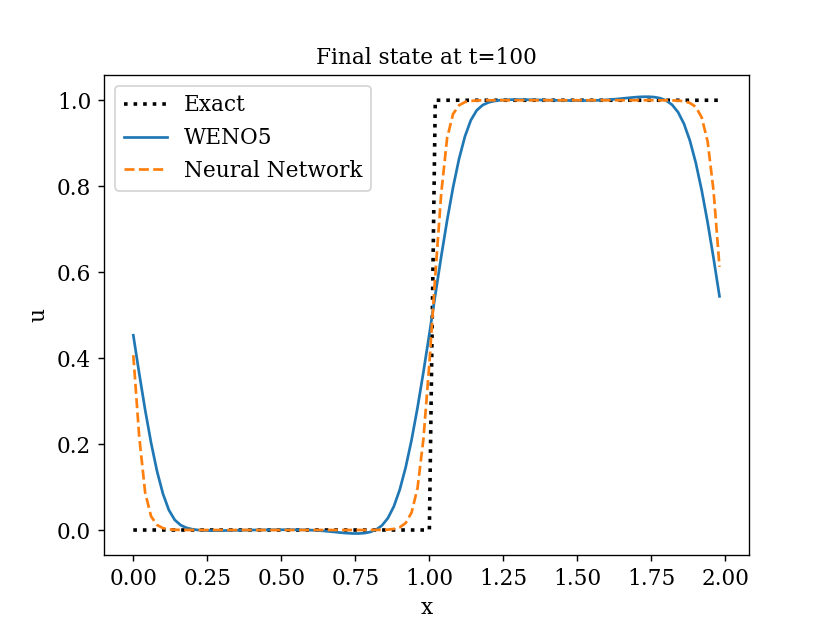
\includegraphics[width=0.62\textwidth]{step_advection/final_snapshot.png}
\caption{Advection d'un créneau périodique à $t=100$ ($L=2$, 100 cellules,
CFL$=2/3$). Le réseau reconstruit le front se déplaçant vers la droite de
façon plus nette que WENO5, mais dépasse légèrement au front gauche.}
\end{figure}

\textbf{Advection d'un créneau} (Sec.~4.1 de l'article)~: WENO5-NN réduit
l'erreur $L_1$ de 28,7\%, $L_2$ de 17,1\%, $L_\infty$ de 5,2\%, et la
largeur du choc de 21,4\%, par rapport à WENO5 classique -- la victoire la
plus nette et la plus cohérente des trois cas de test, reproduisant
directement le résultat revendiqué par l'article.

\textbf{Équation de Burgers} (Sec.~4.2)~: un résultat réellement mitigé.
WENO5-NN l'emporte sur 3 des 4 résolutions de grille testées, en erreur
$L_2$ par rapport à une solution de référence fine, et perd sur la
quatrième. Cela correspond à l'observation de l'article lui-même, selon
laquelle les deux schémas se comportent de façon similaire pour un vrai
choc, l'avantage du réseau provenant surtout de la région lisse avant le
choc.

\begin{figure}[htbp]
\centering
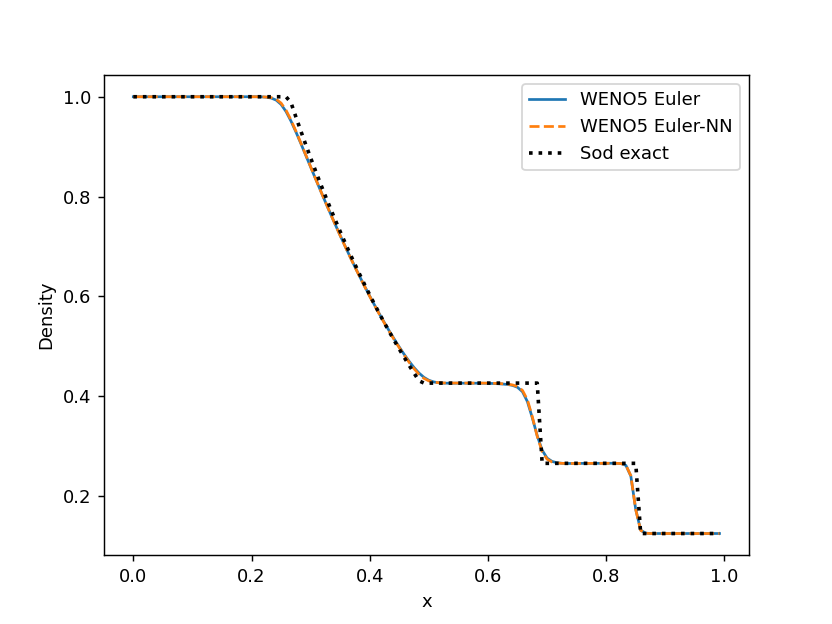
\includegraphics[width=0.5\textwidth]{sod/density_final.png}
\caption{Profil de densité du tube à choc de Sod (120 cellules)~: WENO5,
WENO5-NN et la solution exacte de Riemann sont visuellement
indiscernables.}
\end{figure}

\textbf{Sod et Shu--Osher} (Euler, Sec.~4.3)~: une quasi-égalité, mais
techniquement une défaite pour le réseau selon le critère strict
\texttt{beats\_teacher} -- l'erreur $L_\infty$ par rapport à la solution
réelle est supérieure de $0,265\%$ pour Sod et de $0,551\%$ pour
Shu--Osher. Reproduire la configuration publiée par l'article (300
cellules, $T=2$) retrouve bien sa revendication qualitative de diffusion
post-choc réduite sur Shu--Osher, mais la comparaison numérique stricte
par rapport à la solution réelle/de référence utilisée dans tout ce
rapport ne montre pas de victoire nette à cette résolution.

Le verdict global du Volet~1 est une égalité fortement dépendante du
problème~: une victoire nette sur le problème d'advection/créneau lisse
bien couvert par la distribution d'entraînement de ce réseau, et une
quasi-égalité défavorable sur les deux problèmes (vrai choc de Burgers,
Euler) qui le sollicitent davantage.

% ============================================================
\section{Volet 2~: NN-TENO5 (entraîné par imitation) vs.\ TENO5}
\label{sec:volet2}

La deuxième phase reprend la même idée pour TENO5~: un réseau
classifieur, entraîné à reproduire la décision garder/écarter propre de
TENO5 pour chaque candidat, à partir des mêmes données d'entrée.
Concrètement, \texttt{build\_teno\_network}
(\texttt{src/networks/TenoNetworks.py}) est un perceptron multicouche à
cinq couches de poids, suivant une architecture de type NENO~: un stencil
normalisé à 5 valeurs en entrée, quatre couches cachées ReLU de largeur
décroissante (64, 32, 16, 8), et une dernière couche sigmoïde produisant
une probabilité de trouble par candidat de TENO5 (3 pour les trois
candidats de TENO5).

\begin{figure}[htbp]
\centering
\resizebox{\textwidth}{!}{%
\begin{tikzpicture}[
  every node/.style={font=\small},
  iobox/.style={draw, thick, minimum width=0.75cm, minimum height=0.5cm, inner sep=1pt},
  bigbox/.style={draw, thick, minimum width=1.5cm, minimum height=1.3cm},
  smallbox/.style={draw, thick, minimum width=0.9cm, minimum height=0.6cm},
  stripe/.style={draw, thin, minimum width=0.5cm, minimum height=0.28cm, inner sep=0pt},
]

\foreach \i/\lab/\y in {1/u_{i-2}/1.1, 2/u_{i-1}/0.55, 3/u_i/0, 4/u_{i+1}/-0.55, 5/u_{i+2}/-1.1}{
  \node[iobox] (in\i) at (0,\y) {$\lab$};
}
\node at (0,1.75) {$X^0$};

\node[bigbox] (h1) at (2.3,0) {$W^1 \oplus b^1$};
\node at (2.3,-1.0) {\footnotesize 64 neurones};
\node at (2.3,1.0) {\footnotesize $Y^1{=}W^1X^0{+}b^1$};
\foreach \i in {1,...,5}{
  \draw[-latex] (in\i.east) -- (h1.west);
}

\node[smallbox] (relu1) at (4.0,0) {$\sigma^{\text{RELU}}$};
\draw[-latex] (h1.east) -- (relu1.west);

\foreach \k/\y in {1/1.5,2/1.15,3/0.8,4/0.45,5/0.1,6/-0.25,7/-0.6,8/-0.95,9/-1.3}{
  \node[stripe] (x1-\k) at (5.4,\y) {};
}
\node at (5.4,1.9) {$X^1$};
\draw[-latex] (relu1.east) -- (x1-1.west);
\draw[-latex] (relu1.east) -- (x1-9.west);

\node at (6.6,0) {\Large $\cdots$};

\foreach \k/\y in {1/1.1,2/0.75,3/0.4,4/0.05,5/-0.3,6/-0.65,7/-1.0}{
  \node[stripe] (x4-\k) at (7.8,\y) {};
}
\node at (7.8,1.5) {$X^4$};

\node[bigbox] (h5) at (9.9,0) {$W^5 \oplus b^5$};
\node at (9.9,-1.0) {\footnotesize 3 neurones};
\node at (9.9,1.0) {\footnotesize $Y^5{=}W^5X^4{+}b^5$};
\draw[-latex] (x4-1.east) -- (h5.west);
\draw[-latex] (x4-7.east) -- (h5.west);

\node[smallbox] (sig) at (11.6,0) {$\sigma^{\text{sig}}$};
\draw[-latex] (h5.east) -- (sig.west);

\foreach \i/\lab/\y in {1/p^1/0.6,2/p^2/0,3/p^3/-0.6}{
  \node[iobox] (out\i) at (13.0,\y) {$\lab$};
  \draw[-latex] (sig.east) -- (out\i.west);
}
\node at (13.0,1.2) {$Y^{\text{out}}$};

\node at (0,-2.1) {Couche d'entrée};
\node at (3.15,-2.1) {Couche cachée 1};
\node at (7.2,-2.1) {Couches cachées 2,3,4};
\node at (11.3,-2.1) {Couche de sortie};

\end{tikzpicture}}
\caption{Architecture du classifieur NN-TENO5~: un stencil normalisé à 5
valeurs $X^0$ alimente quatre couches cachées ReLU de largeur décroissante
(64, 32, 16, 8 neurones) puis une dernière couche sigmoïde, produisant une
probabilité de trouble $p^k$ par candidat de TENO5.}
\end{figure}

Chaque couche $l=1,\dots,5$ calcule la même application affine avant
activation, $X^{l-1} \to Y^l = w^l X^{l-1} + b^l$, où $w^l$ et $b^l$ sont
la matrice de poids et le vecteur de biais propres à cette couche. Les
quatre couches cachées utilisent l'activation ReLU, et la couche de
sortie une sigmoïde pour projeter dans $[0,1]$~:
\[
\sigma^{\text{RELU}}(x) = \max(x, 0), \qquad
\sigma^{\text{sig}}(x) = \frac{1}{1+e^{-x}}.
\]
Le résultat $Y^{\text{out}} = [p^1,p^2,p^3]$ se lit directement comme la
probabilité que chaque candidat soit traversé par une discontinuité~: à
l'inférence, le wrapper TENO5 déterministe écarte un candidat dès que sa
probabilité dépasse \texttt{DEFAULT\_NEURAL\_THRESHOLD}$=0{,}5$
(\texttt{src/schemes/teno5.py}), reprenant exactement la règle de
décision à 50\% de NENO6, même si pendant l'entraînement par perte
physique déroulée ce seuil dur est remplacé par la probabilité continue
elle-même, afin que les gradients puissent traverser la décision
(section~\ref{sec:jax}).

Par construction, un réseau entraîné uniquement à imiter la décision d'un
maître ne peut pas dépasser la qualité de reconstruction de ce maître, si
ce n'est par sa propre erreur de lissage/généralisation -- aucun
mécanisme de l'entraînement par imitation ne peut le pousser
\emph{au-delà} du schéma qu'il copie. Ceci est confirmé directement plutôt
que simplement supposé~:

\begin{itemize}
    \item Sur 3 des 4 benchmarks scalaires testés, NN-TENO5 produit une
    égalité \emph{exacte} avec TENO5 -- le réseau reproduit la décision
    identique, jusqu'au dernier chiffre mesuré.
    \item Sur l'advection d'un créneau, il perd de $0,64\%$ -- une petite
    erreur de généralisation par rapport à son maître.
    \item Sur les benchmarks Euler, il produit deux petites victoires
    selon le critère strict (section~\ref{sec:consolide}), ce qui est
    compatible avec le plafond de l'imitation~: reproduire ou perturber
    très légèrement la décision du maître peut occasionnellement se
    rapprocher un peu plus de la solution réelle par hasard, et non par
    amélioration systématique.
\end{itemize}

Deux tentatives ultérieures (documentées dans \texttt{Results.md} comme
Phases 2 à 9) ont essayé de dépasser ce plafond tout en restant dans le
paradigme de l'imitation~: entraînement sur un jeu de données à cible
exacte, extension à un stencil à 7 points de type WENO7, une recherche
d'hyperparamètres poussée, et entraînement sur des données TENO5
réétiquetées par un « oracle » conçu pour récompenser de véritables
meilleures décisions. Chacune de ces tentatives a produit soit un résultat
négatif, soit une petite victoire qui plafonne au même type de limite --
confirmant que ce plafond est structurel à l'entraînement par imitation
lui-même, et non un simple manque de réglage. Ce constat a directement
motivé la seconde et plus grande phase du stage.

% ============================================================
\section{Motivation d'un nouveau paradigme d'entraînement}

Le plafond du Volet~2 a une cause précise~: la fonction de perte d'un
réseau entraîné par imitation ne mesure jamais que la distance à la
décision du \emph{maître}, jamais la distance à la \emph{solution réelle}.
Un réseau ne peut pas être poussé vers une réponse qu'on ne lui montre
jamais. Dépasser réellement TENO5 nécessite donc un signal d'entraînement
fondamentalement différent -- un signal qui juge le réseau par rapport à
la réalité, et non par rapport au schéma classique.

C'est exactement ce que l'encadrant académique du stage a proposé sous le
nom de \textbf{fonction de perte physique déroulée} (Unrolled Physics
Loss)~: plutôt qu'une étiquette d'imitation ponctuelle par stencil, faire
tourner le réseau sur $K$ pas de simulation réels et calculer une perte
directement par rapport à la solution réelle $K$ pas plus tard. Comme
l'ensemble du déroulement doit être différentié, cette proposition ne
pouvait tout simplement pas être testée dans le code NumPy/Keras
d'origine~: elle a nécessité la construction, à partir de zéro, d'une
nouvelle pile numérique entièrement différentiable
(section~\ref{sec:jax}).

\begin{figure}[htbp]
\centering
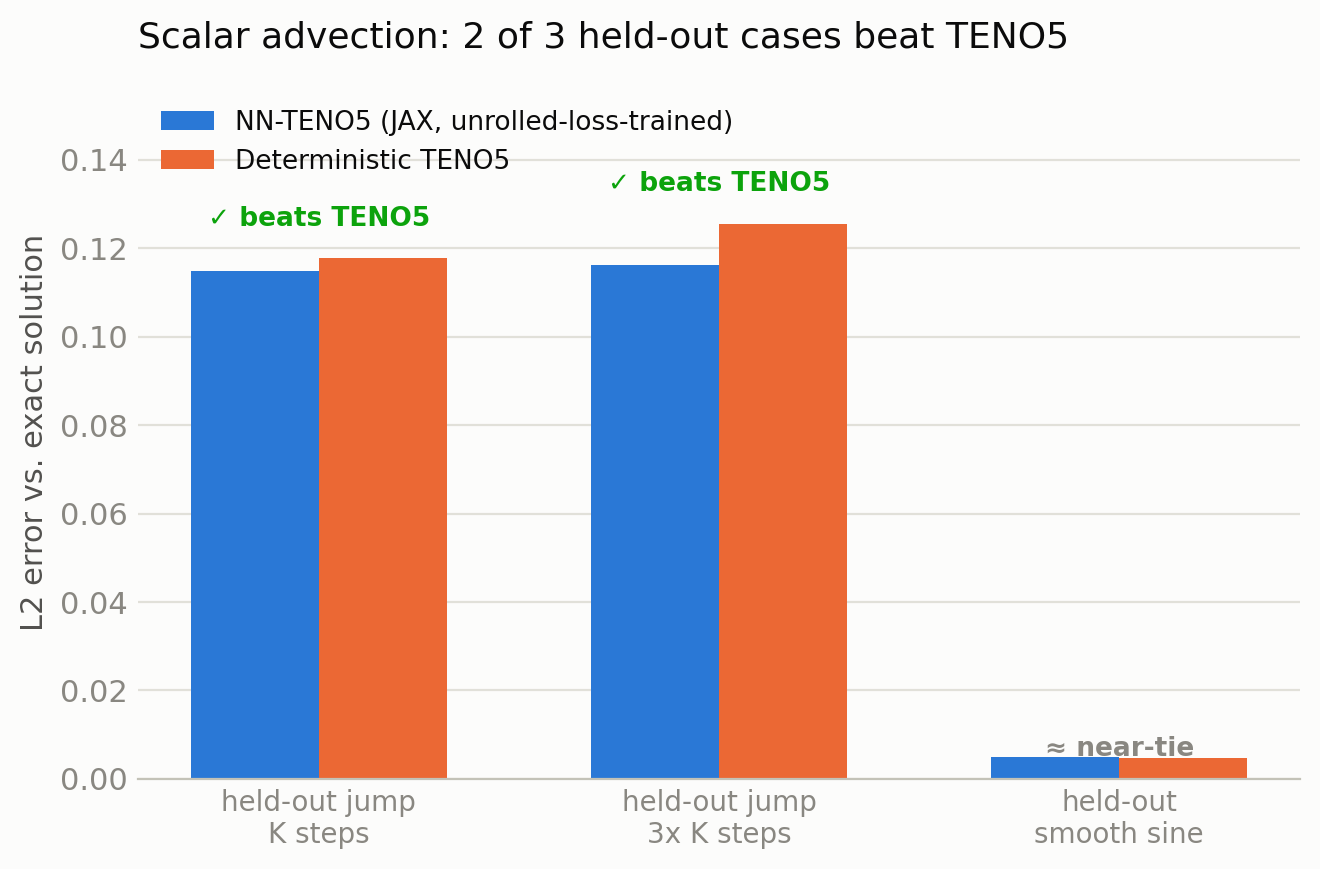
\includegraphics[width=0.62\textwidth]{02_scalar_beats_teacher.png}
\caption{Premier signal positif pour le nouveau paradigme (Phase~10)~: un
réseau entraîné avec la perte déroulée bat TENO5 sur 2 des 3 cas
d'advection scalaire mis de côté -- un résultat que l'entraînement par
imitation ne peut structurellement pas produire.}
\end{figure}

Ce premier résultat était étroit -- une victoire seulement sur des cas mis
de côté ressemblant à la forme et à l'horizon temporel propres à la
distribution d'entraînement -- et ne se généralisait pas encore aux
benchmarks canoniques à pleine échelle ni au système d'Euler. Le reste du
stage (sections~\ref{sec:jax} à~\ref{sec:instabilite}) consiste à
transformer ce signal étroit en une victoire vérifiée, à l'échelle des
benchmarks canoniques.

% ============================================================
\section{La fonction de perte physique déroulée~: formulation}
\label{sec:perte}

La perte entraîne le réseau en comparant un déroulement réel sur $K$ pas à
la solution réelle, plutôt qu'une seule décision de stencil à une
étiquette de maître~:
\[
L = \lambda_1 L_{\text{MSE}} + \lambda_2 L_{\text{TV}}
  + \lambda_3 L_{\text{BVD}} + \lambda_4 L_{\text{Reg}},
\]
\begin{align*}
L_{\text{MSE}} &= \frac{1}{N}\sum_i \left(u_i^{(n+K)} - u_{i,\text{exact}}^{(n+K)}\right)^2, \\
L_{\text{TV}} &= \max\!\left(0,\ \mathrm{TV}(u^{(n+K)}) - \mathrm{TV}(u^{(n)})\right),
\quad \mathrm{TV}(v) = \sum_i |v_{i+1}-v_i|, \\
L_{\text{BVD}} &= \mathrm{moyenne}\!\left(\max\!\left(0,\ BV_{\text{réseau}} - BV_{\text{TENO5}}\right)\right), \\
BV(\Phi)_{i+1/2} &= \left|\Phi_i(x_{i+1/2}) - \Phi_{i+1}(x_{i+1/2})\right|, \\
L_{\text{Reg}} &= \left\| c_{\text{RN}} - c_{\text{base}} \right\|^2.
\end{align*}

$L_{\text{MSE}}$ est l'erreur physique directe après $K$ pas.
$L_{\text{TV}}$ pénalise toute augmentation de la variation totale au
cours du déroulement -- une pénalité anti-oscillation de Gibbs qui ne
nécessite pas de connaître la solution réelle. $L_{\text{BVD}}$, tiré
directement du principe de Boundary Variation Diminishing de Fu, Hu \&
Adams (sa forme précise n'était pas pleinement spécifiée dans la
proposition d'origine et a été confirmée avec l'encadrant académique),
pénalise le réseau uniquement lorsque sa propre reconstruction
d'interface est \emph{moins} cohérente avec sa voisine que ne le serait
la reconstruction propre de TENO5 -- un signal de cohérence différentiable,
interface par interface. $L_{\text{Reg}}$ ancre les poids de
reconstruction du réseau $c_{\text{RN}}$ vers les poids linéaires
optimaux propres de TENO5, $c_{\text{base}} = [1/10,\,3/5,\,3/10]$,
réutilisant une technique déjà validée lors de l'entraînement par
imitation (section~\ref{sec:volet2}) pour empêcher le réseau de dériver
arbitrairement loin d'un point de départ connu comme bon.

Pour le système d'Euler, un cinquième terme, une pénalité de positivité, a
été ajouté au cours de ce stage (absent de la proposition d'origine) après
que la Phase~13 a établi qu'il était structurellement nécessaire à un
entraînement stable (section~\ref{sec:instabilite}).

% ============================================================
\section{La réécriture différentiable en JAX}
\label{sec:jax}

Entraîner à travers un déroulement de $K$ pas exige que chaque opération
de ce déroulement -- reconstruction, calcul du flux, avancement temporel
-- soit différentiable de bout en bout. Rien dans le code d'origine ne
satisfait cette exigence~: le solveur NumPy n'a aucune notion de
gradient, et \texttt{model.predict()} de Keras se détache entièrement de
tout graphe de gradient. \texttt{src/differentiable/} est donc une
réécriture JAX complète du c\oe{}ur numérique du projet, et non une simple
enveloppe autour de l'existant.

\begin{table}[htbp]
\begin{adjustbox}{max width=\textwidth, center}
\begin{tabular}{ll}
\toprule
\textbf{Module} & \textbf{Ce qu'il porte} \\
\midrule
\texttt{teno5\_jax.py} & Les calculs de candidats/régularité/sélection de
TENO5, plus une reconstruction souple (poids de conservation continu) à
travers laquelle un réseau peut être entraîné \\
\rowrule
\texttt{numerics\_jax.py} & Le solveur scalaire en volumes finis -- un
déroulement basé sur \texttt{jax.lax.scan}, et la véritable construction
BVD \\
\rowrule
\texttt{euler\_jax.py} & Le solveur d'Euler caractéristique complet --
base propre de Roe, séparation de flux, réparation de positivité \\
\rowrule
\texttt{projection\_jax.py} & Convertit la probabilité brute de trouble
produite par le réseau en un poids de reconstruction (souple pour
l'entraînement, seuillé pour l'inférence), et implémente le mécanisme de
mélange convexe de la section~\ref{sec:volet4} \\
\rowrule
\texttt{losses\_jax.py} & Les quatre termes de la fonction de perte
déroulée, plus la pénalité de positivité pour Euler \\
\rowrule
\texttt{teno5\_jax\_toy.py} & Un MLP JAX de même architecture que
NN-TENO5, utilisé pour l'entraînement -- pas un portage direct du point de
sauvegarde Keras entraîné \\
\bottomrule
\end{tabular}
\end{adjustbox}
\caption{Contenu de \texttt{src/differentiable/}.}
\end{table}

Chaque portage est testé en régression contre le solveur NumPy/Keras
d'origine à la précision float64, et non par simple concordance visuelle,
avant tout entraînement -- c'est ce qui permet de garantir qu'un résultat
d'entraînement reflète la physique et non un écart d'implémentation
silencieux entre les deux piles.

\begin{figure}[htbp]
\centering
\begin{tikzpicture}
\node[rbox=6.2cm] (n1) {Tirer une condition initiale et une longueur de
déroulement $K$};
\node[rbox=6.2cm, below=0.55cm of n1] (n2) {Dérouler $K$ pas SSPRK3, en
utilisant la reconstruction du réseau à chaque sous-étape};
\node[rbox=6.2cm, below=0.55cm of n2] (n3) {Comparer l'état au pas
$n{+}K$ à la solution réelle};
\node[rbox=6.2cm, below=0.55cm of n3] (n4) {Calculer
$L=\lambda_1 L_{\text{MSE}}+\lambda_2 L_{\text{TV}}+\lambda_3 L_{\text{BVD}}+\lambda_4 L_{\text{Reg}}$};
\node[rbox=6.2cm, below=0.55cm of n4] (n5) {Rétropropager à travers les
$K$ pas (\texttt{jax.lax.scan})};
\node[rbox=6.2cm, below=0.55cm of n5] (n6) {Mettre à jour les paramètres
du réseau (Adam, avec écrêtage du gradient)};

\draw[flow] (n1) -- (n2);
\draw[flow] (n2) -- (n3);
\draw[flow] (n3) -- (n4);
\draw[flow] (n4) -- (n5);
\draw[flow] (n5) -- (n6);
\draw[flow] (n6.east) -- ++(1.3,0) |- (n1.east);
\end{tikzpicture}
\caption{La boucle d'entraînement de la fonction de perte physique
déroulée.}
\end{figure}

% ============================================================
\section{Volet 3~: benchmarks scalaires (advection et Burgers)}
\label{sec:volet3}

La fonction de perte physique déroulée a d'abord été testée sur
l'advection scalaire et l'équation de Burgers, toutes deux disposant de
solutions de référence exactes ou bien convergées, sans la complexité
supplémentaire du conditionnement de base propre. Trois obstacles ont dû
être résolus successivement avant d'obtenir une victoire canonique~:

\begin{enumerate}
    \item Entraîner littéralement selon les équations de la proposition,
    avec des termes $L_{\text{TV}}$ et $L_{\text{Reg}}$ bruts, non
    normalisés, laissait le gradient de $L_{\text{TV}}$ dominer celui de
    $L_{\text{MSE}}$ d'un facteur d'environ $4\times$ -- corrigé en
    normalisant les deux termes.
    \item Entraîner un réseau initialisé aléatoirement directement contre
    la perte déroulée échouait franchement, perdant chaque test mis de
    côté -- corrigé par un pré-entraînement par imitation (la propre
    méthode du Volet~2), suivi d'un affinage avec la perte déroulée, en
    réutilisant le même schéma de démarrage-à-chaud-puis-ancrage déjà
    validé à cet endroit.
    \item Le réseau obtenu (Phase~10, section précédente) gagnait sur 2
    des 3 tests mis de côté, mais ne se généralisait ni au benchmark
    canonique à pleine échelle, ni au flux non linéaire de Burgers, absent
    de la distribution d'entraînement.
\end{enumerate}

Le correctif final (Phase~19) a consisté à réutiliser un mécanisme
développé d'abord pour le système d'Euler (section~\ref{sec:volet4})~:
une petite \emph{tête de mélange}, entraînée séparément, qui produit un
coefficient de combinaison convexe $\lambda \in [0,1]$ entre la
reconstruction propre de TENO5 et celle du réseau,
\[
u_{\text{final}} = (1-\lambda)\, u_{\text{TENO5}} + \lambda\, u_{\text{réseau}},
\]
combiné à des exemples d'entraînement explicites sur le flux de Burgers,
absents du jeu d'entraînement scalaire d'origine. Ce mécanisme garantit
que le réseau ne peut qu'interpoler \emph{vers} sa propre reconstruction
depuis celle de TENO5, jamais la dépasser dans le mauvais sens -- et,
fait notable, la tête non entraînée (avec un biais initial prudent
donnant $\lambda \approx 4,7\%$ uniformément) gagnait déjà sur les deux
benchmarks canoniques \emph{avant tout entraînement supplémentaire}, une
véritable surprise qui a révélé un second résultat~: un mélange uniforme
bat un mélange concentré sur les zones à problème (pondérer le réseau
uniquement là où le schéma classique signale un stencil à problème), car
il permet aussi au réseau de corriger les petites erreurs du schéma
classique dans les régions par ailleurs lisses.

Le résultat final, à l'échelle canonique (\texttt{ValidationMatrix\_ProjPDF.py}, 128 pas pour l'advection, 64 pour Burgers), est présenté au
tableau~\ref{tab:volet3} de la section~\ref{sec:consolide}~: une victoire
vérifiée sur les deux benchmarks, y compris Burgers -- explicitement hors
de la distribution d'entraînement.

% ============================================================
\section{Volet 4~: le système d'Euler (Sod et Shu--Osher)}
\label{sec:volet4}

Le système d'Euler est plus difficile pour deux raisons indépendantes~:
c'est une reconstruction couplée, caractéristique, plutôt que scalaire
(section~\ref{sec:fond-vf}), et il doit rester physiquement valide
(densité et pression positives) à chaque étape intermédiaire de
l'entraînement, pas seulement à convergence. La section~\ref{sec:instabilite}
détaille la défaillance de stabilité que cela a causée~; cette section
présente le résultat de précision une fois l'entraînement rendu stable.

Le mécanisme qui a finalement produit une victoire canonique est le même
mélange convexe introduit à la section~\ref{sec:volet3}, mais son
coefficient $\lambda$ a dû être calculé par une tête \emph{dédiée},
entraînée séparément, plutôt que réutilisé depuis la propre sortie de
probabilité de trouble du réseau. Réutiliser ce signal (Phase~17) faisait
jouer à $\lambda$ deux rôles incompatibles à la fois -- signaler le
trouble \emph{et} calibrer la confiance à accorder au réseau -- et
l'entraîner directement à travers ce signal a causé trois régressions
distinctes. Une petite tête entraînée spécifiquement pour calibrer
$\lambda$, initialisée prudemment (biais $=-3$, soit $\lambda \approx
4,7\%$ au départ), a corrigé ce problème et produit la première victoire
canonique nette du projet (Phase~18)~:

\begin{figure}[htbp]
\centering
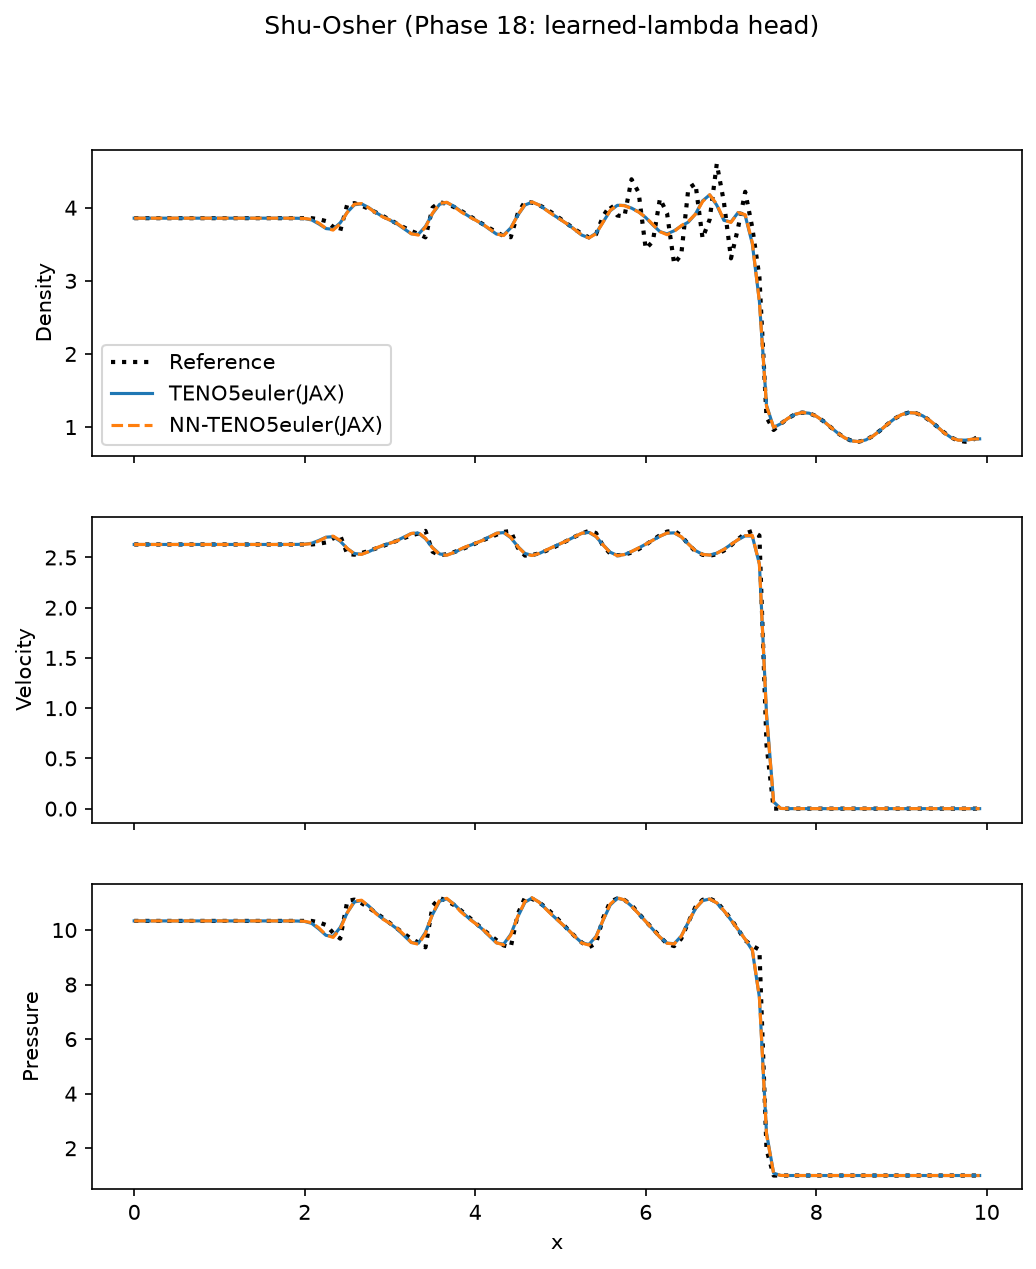
\includegraphics[width=0.55\textwidth]{euler_jax_comparison/shu_osher_phase18.png}
\caption{Shu--Osher (Phase~18, tête de mélange dédiée)~: NN-TENO5euler et
TENO5euler sont visuellement quasi identiques par rapport à la référence,
NN-TENO5euler étant $1,84\%$ plus précis en $L_1$ moyen sur les trois
variables conservées.}
\end{figure}

Sod, en revanche, reste une quasi-égalité légèrement défavorable au réseau
même après ce correctif. Deux tentatives supplémentaires (Phases~20--21)
-- un taux d'apprentissage 50 fois plus élevé pour la seule tête de
mélange, puis une tête enrichie recevant directement le stencil brut
plutôt que le seul résumé de probabilité de trouble -- ne déplacent le
rapport de Sod que marginalement ($1,0045\times$, puis $1,0026\times$),
sans jamais dépasser la parité. Un balayage direct d'un coefficient de
mélange fixe (non appris) $\lambda$ confirme qu'il s'agit d'une véritable
limite structurelle de la reconstruction propre du réseau sur Sod, et non
d'un problème de calibration~: l'erreur de Sod augmente de façon
\emph{monotone} pour chaque $\lambda$ testé de $0$ à $0,3$, tandis que
l'erreur de Shu--Osher \emph{diminue} de façon monotone jusqu'à
$\lambda \approx 0,2$ sur ce même balayage. Aucun réglage de la tête de
mélange ne peut corriger un tronc qui, sur ce problème précis, est tout
simplement moins précis que TENO5 lui-même.

La progression complète depuis le premier point de sauvegarde stable
jusqu'à ce résultat est présentée au tableau~\ref{tab:progression} de la
section~\ref{sec:consolide}.

% ============================================================
\section{Stabilité numérique~: diagnostic et correction de l'instabilité d'Euler}
\label{sec:instabilite}

La première tentative d'entraîner le système d'Euler à travers la
fonction de perte physique déroulée a franchement divergé~: les valeurs
d'état croissaient sans limite en quelques sous-pas SSPRK3, quelle que
soit l'intensité de la dissipation de la séparation de flux de
Lax--Friedrichs.

\begin{figure}[htbp]
\centering
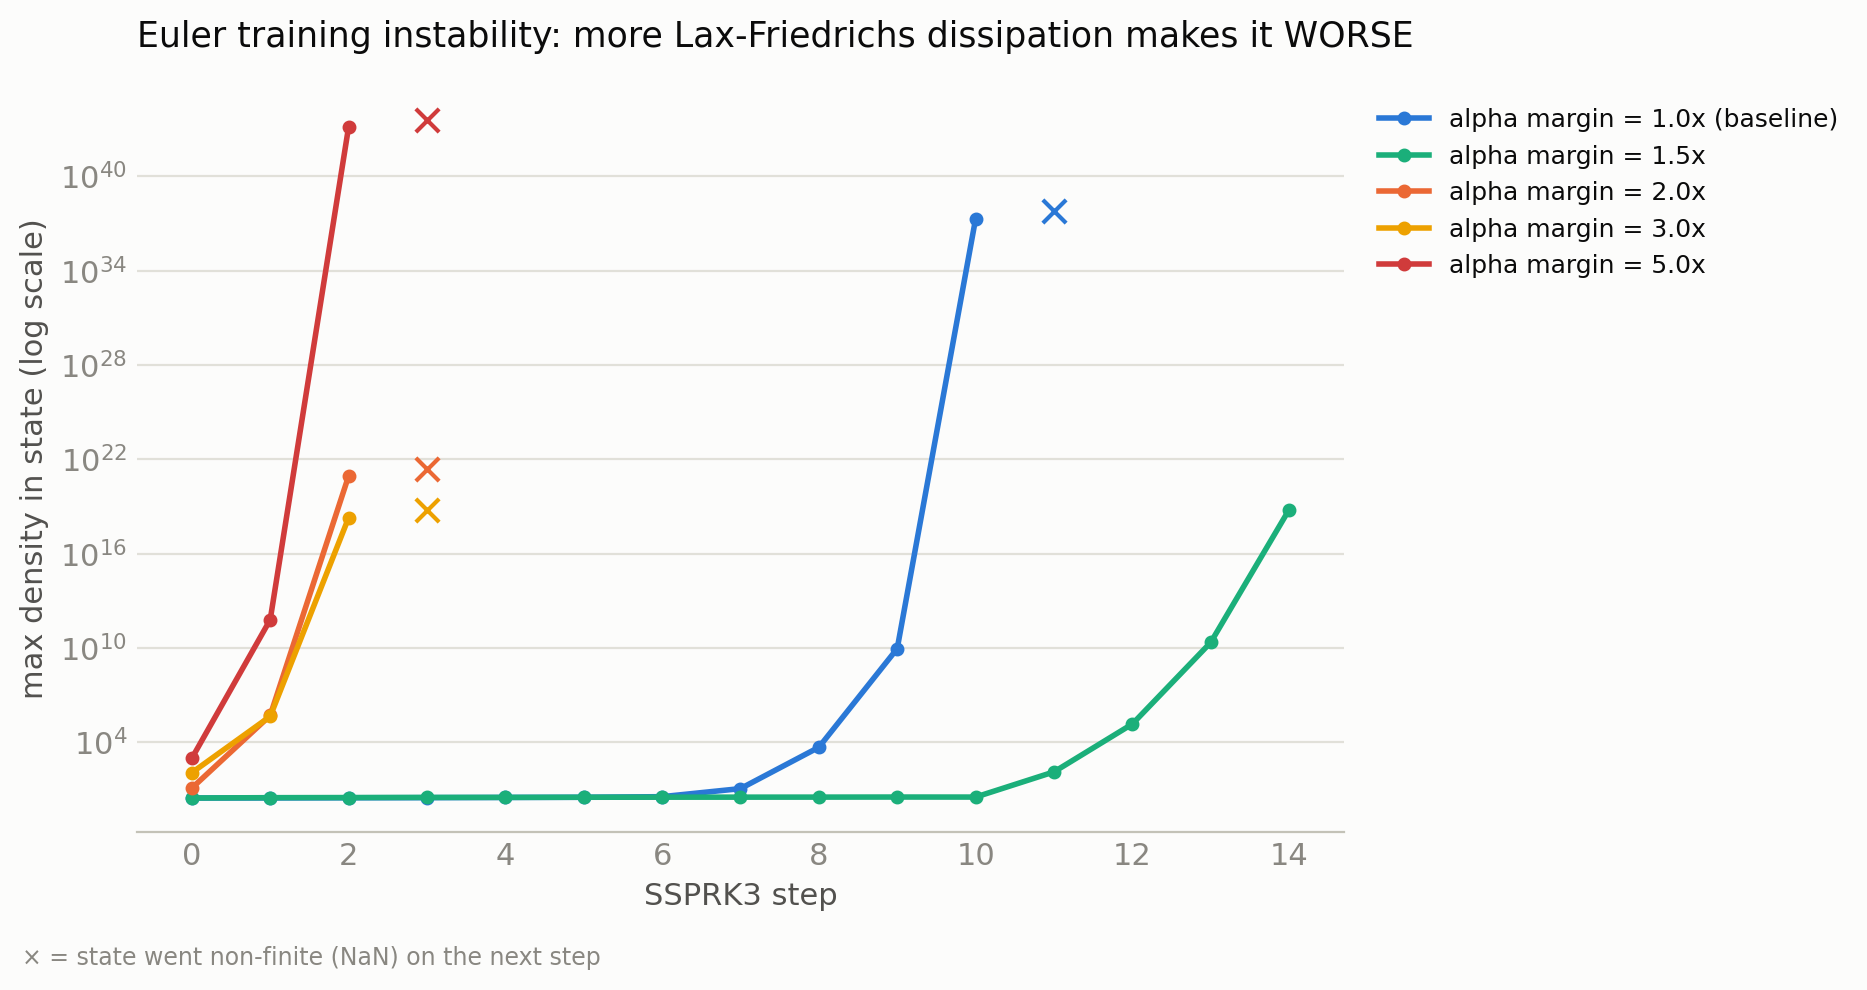
\includegraphics[width=0.72\textwidth]{04_euler_instability.png}
\caption{Augmenter la dissipation fait arriver l'instabilité \emph{plus
vite}, pas plus lentement -- une signature qui exclut un manque de
dissipation numérique comme cause.}
\end{figure}

Ce résultat contre-intuitif -- davantage de dissipation aggravant, et non
améliorant, la situation -- a été l'indice diagnostique clé. Il écartait
une instabilité ordinaire de choc sous-résolu, et orientait vers un bug
dans le traitement des violations de positivité. Deux défauts concrets ont
été identifiés et corrigés durant ce stage~:

\begin{enumerate}
    \item \textbf{Une pénalité de positivité structurellement inerte.} Le
    terme de perte censé pénaliser les états non physiques (densité ou
    pression négatives) était calculé sur l'état final \emph{déjà
    réparé} de chaque pas, après qu'un plancher/écrêtage strict avait déjà
    été appliqué -- il ne pouvait donc mathématiquement jamais être non
    nul, quelle que soit la gravité de la violation de positivité avant
    réparation. Corrigé en calculant la pénalité sur les sous-étapes
    avant réparation, dans une nouvelle fonction
    \texttt{rollout\_with\_\allowbreak positivity\_\allowbreak penalty}.
    \item \textbf{Un mécanisme de réparation incomplet.} L'étape de
    réparation ne vérifiait qu'un signe négatif~; elle ne vérifiait ni les
    valeurs non finies (\texttt{NaN}/\texttt{Inf}), ni une magnitude non
    bornée, deux situations pouvant provenir d'une reconstruction
    neuronale évolutive et imparfaite qui se répercute sur la base propre
    de Roe du pas \emph{suivant}. Corrigé en ajoutant des vérifications
    explicites de finitude et de magnitude au masque de réparation, et en
    écrêtant (et non plus seulement en plafonnant) la densité et la
    pression.
\end{enumerate}

Combinés à la clarification propre de l'encadrant académique sur la
définition correcte de $L_{\text{BVD}}$ (section~\ref{sec:perte}) et à un
passage à un moyennage des voisins plutôt qu'à un simple écrêtage aveugle
pour les violations de positivité isolées, ces correctifs ont produit le
premier entraînement Euler qui ne diverge pas (Phase~13), et ont
mesurablement amélioré chaque tentative d'entraînement suivante. Ils
n'ont cependant pas, à eux seuls, produit de victoire canonique -- celle-ci
a nécessité la tête de mélange dédiée de la section~\ref{sec:volet4},
par-dessus une procédure d'entraînement stable.

Une première tentative de reproduction d'une amélioration par mélange de
données lisses (Phase~14) a également corrompu franchement un bon point
de sauvegarde, pour une seconde cause, indépendante~: l'absence
d'écrêtage de la norme du gradient. Un unique lot anormal a produit un pic
de perte catastrophique qui a écrasé le bon point de sauvegarde avant
qu'il ne soit remarqué. \texttt{optax.clip\_by\_global\_norm(1.0)} a
depuis été adopté comme pratique standard pour chaque script
d'entraînement, avec en complément un suivi du meilleur point de
sauvegarde par validation (réévaluation périodique contre la solution
réelle pendant l'entraînement, en conservant les meilleurs paramètres
observés plutôt que seulement les derniers).

% ============================================================
\section{Métriques d'évaluation}
\label{sec:metriques}

Chaque résultat de ce rapport est mesuré avec le même ensemble fixe de
métriques, appliqué identiquement au schéma classique et au réseau. Soit
$u_i$ la valeur de cellule d'un schéma et $u_i^{\text{ref}}$ la solution
réelle à la même cellule, avec $d_i = u_i - u_i^{\text{ref}}$~:
\[
L_1 = \frac{1}{N}\sum_i |d_i|, \qquad
L_2 = \sqrt{\frac{1}{N}\sum_i d_i^2}, \qquad
L_\infty = \max_i |d_i|.
\]
Pour le système d'Euler, ces normes sont calculées indépendamment pour
chaque variable conservée (densité, quantité de mouvement, énergie) puis
moyennées en un unique scalaire $\bar L_1$ pour les comparaisons
générales.

Trois diagnostics supplémentaires, spécifiques à Euler ou aux
discontinuités, complètent le tableau~:

\begin{itemize}
    \item \textbf{Variation totale} $\mathrm{TV}(u)=\sum_i|u_{i+1}-u_i|$~:
    dépasser la variation totale propre de la solution réelle signale une
    oscillation parasite de type Gibbs introduite par le schéma.
    \item \textbf{Positivité} (Euler uniquement)~: $\min_i \rho_i > 0$ et
    $\min_i p_i > 0$ -- un critère booléen de validité physique,
    indépendant de toute norme d'erreur.
    \item \textbf{Erreur de localisation du choc/contact}~: la distance
    entre la position du plus fort gradient de densité propre au schéma et
    celle de la solution réelle, séparément pour le choc et (en dehors
    d'une petite fenêtre d'exclusion autour de celui-ci) pour la
    discontinuité de contact.
\end{itemize}

Un résultat n'est rapporté comme une \textbf{victoire} que selon le
critère strict introduit à la section~5 ($L^{\text{RN}} \le
L^{\text{classique}}$ par rapport à la solution réelle) -- jamais selon le
critère plus souple \texttt{teacher\_fidelity}, utilisé uniquement pour un
petit nombre de tests d'acceptation précoces et explicitement jamais
traité comme une preuve de supériorité dans ce rapport.

% ============================================================
\section{Résultats consolidés}
\label{sec:consolide}

\begin{table}[htbp]
\begin{adjustbox}{max width=\textwidth, center}
\begin{tabular}{lrrrl}
\toprule
\textbf{Benchmark} & \textbf{TENO5} & \textbf{NN-TENO5 (JAX)} & \textbf{Rapport} & \textbf{Verdict} \\
\midrule
Advection ($L_1$) & 3,4819e-02 & 3,3813e-02 & $0,9711\times$ & \textbf{VICTOIRE} \\
\rowrule
Advection ($L_2$) & 9,8960e-02 & 9,5521e-02 & $0,9653\times$ & \textbf{VICTOIRE} \\
\rowrule
Burgers ($L_1$, hors distribution) & 2,0697e-04 & 1,7873e-04 & $0,8636\times$ & \textbf{VICTOIRE} \\
\rowrule
Burgers ($L_2$, hors distribution) & 8,1670e-04 & 6,6493e-04 & $0,8142\times$ & \textbf{VICTOIRE} \\
\bottomrule
\end{tabular}
\end{adjustbox}
\caption{Volet 3 (scalaire), évaluation à l'échelle canonique. NN-TENO5
(JAX) gagne sur les deux benchmarks, y compris Burgers, explicitement
hors de la distribution d'entraînement.\label{tab:volet3}}
\end{table}

\begin{table}[htbp]
\begin{adjustbox}{max width=\textwidth, center}
\begin{tabular}{lrrrl}
\toprule
\textbf{Benchmark} & \textbf{TENO5euler $\bar L_1$} & \textbf{NN-TENO5euler $\bar L_1$} & \textbf{Rapport} & \textbf{Verdict} \\
\midrule
Sod & 8,2583e-03 & 8,2871e-03 & $1,0035\times$ & DÉFAITE \\
\rowrule
Shu--Osher & 2,1319e-01 & 2,0926e-01 & $0,9816\times$ & \textbf{VICTOIRE} \\
\bottomrule
\end{tabular}
\end{adjustbox}
\caption{Volet 4 (Euler), meilleur modèle disponible (tête de mélange
dédiée, Phase~18). Sod est $0,35\%$ moins précis~; Shu--Osher est
$1,84\%$ plus précis -- la première victoire nette contre un schéma
classique sur un benchmark canonique obtenue dans ce projet.}
\end{table}

\begin{table}[htbp]
\begin{adjustbox}{max width=\textwidth, center}
\begin{tabular}{lrr}
\toprule
\textbf{Étape} & \textbf{Rapport Sod} & \textbf{Rapport Shu--Osher} \\
\midrule
Aucun modèle fini pour l'instant & -- & -- \\
\rowrule
Correctif de stabilité (terme de perte mort + bug de réparation) & $1,29\times$ & $1,24\times$ \\
\rowrule
+ données d'entraînement lisses + écrêtage du gradient & $1,16\times$ & $1,23\times$ \\
\rowrule
+ reconstruction à mélange convexe (littérature) & $1,145\times$ & $1,065\times$ \\
\rowrule
+ tête de mélange dédiée, entraînée séparément & $\mathbf{1,003\times}$ & $\mathbf{0,982\times}$ \\
\bottomrule
\end{tabular}
\end{adjustbox}
\caption{Progression sur le système d'Euler à travers plusieurs
correctifs diagnostiqués et vérifiés indépendamment. Un rapport inférieur
à 1 signifie que le réseau est plus précis que TENO5euler.\label{tab:progression}}
\end{table}

\begin{table}[htbp]
\small
\begin{tabularx}{\textwidth}{@{}>{\raggedright\arraybackslash}p{0.24\textwidth}>{\raggedright\arraybackslash}p{0.22\textwidth}>{\centering\arraybackslash}p{0.09\textwidth}>{\raggedright\arraybackslash}X@{}}
\toprule
\textbf{Volet} & \textbf{Verdict} & \textbf{Résultat} & \textbf{Observation principale} \\
\midrule
1. NN-WENO vs.\ WENO & Dépend fortement du problème & ÉGALITÉ & Victoire
sur l'advection d'un créneau et 3/4 des résolutions de Burgers, mais
légère perte sur Sod et Shu--Osher. \\
\rowrule
2. NN-TENO5 (imitation) vs.\ TENO5 & Reproduit principalement le maître &
ÉGALITÉ & Trois égalités exactes sur les benchmarks scalaires, deux
petites victoires sur Euler et une petite perte sur l'advection d'un
créneau. \\
\rowrule
3. NN-TENO5 (perte déroulée), scalaire & Victoire sur les deux benchmarks
canoniques & \textbf{VICTOIRE} & Gain de $3,5\%$ sur l'advection et de
$18,6\%$ sur Burgers (hors distribution), grâce à une tête de mélange
dédiée et un entraînement incluant le flux de Burgers. \\
\rowrule
4. NN-TENO5euler (perte déroulée) & Première victoire canonique nette &
\textbf{VICTOIRE} & Victoire de $1,84\%$ sur Shu--Osher~; Sod reste une
quasi-égalité structurelle légèrement défavorable au réseau. \\
\bottomrule
\end{tabularx}
\caption{Résumé global des quatre volets.}
\end{table}

Chaque variante neuronale, dans chaque volet, tourne aussi nettement plus
lentement par cellule que son équivalent classique -- environ
$5$--$18\times$ pour les modèles basés sur Keras. Les victoires en
précision rapportées ci-dessus ne se traduisent donc pas encore, dans leur
forme actuelle non optimisée, par un avantage en temps de calcul.

% ============================================================
\section{Discussion}

Deux résultats se démarquent comme le principal apport scientifique du
stage, et il s'agit en réalité du même constat vu sous deux angles~: la
\emph{manière} dont un réseau est entraîné détermine le type
d'amélioration réellement atteignable, indépendamment de la capacité du
réseau ou de l'effort de réglage.

Le réseau entraîné par imitation du Volet~2 n'a pu être poussé au-delà de
son maître par aucune recherche d'architecture, aucun réglage
d'hyperparamètres, ni aucun réétiquetage de données (Phases~2 à~9) --
parce que sa fonction de perte ne référence jamais la solution réelle en
premier lieu. Les réseaux des Volets~3 et~4, entraînés directement contre
la solution réelle via la perte déroulée, ont bien franchi ce plafond --
mais seulement une fois deux défauts d'ingénierie distincts et jusque-là
non diagnostiqués (section~\ref{sec:instabilite}) corrigés, et seulement
une fois la sortie propre du réseau contrainte par un mélange convexe
plutôt que pleinement fiabilisée.

Le mécanisme de mélange convexe lui-même mérite une attention
particulière~: il s'est avéré peser plus lourd que n'importe quel
changement d'entraînement testé isolément. Chaque point de sauvegarde
testé avec ce mécanisme s'est amélioré immédiatement, à l'inférence,
\emph{sans aucun réentraînement} (Phase~16) -- le réseau était déjà
suffisamment bon localement pour aider, il fallait simplement l'empêcher
d'être suivi globalement. Entraîner le coefficient de mélange lui-même,
plutôt que de réutiliser un signal existant, a ensuite converti ce gain
d'inférence en les premières véritables victoires canoniques du projet
(Phases~18--19).

Le résultat sur Sod (section~\ref{sec:volet4}) est le constat négatif le
plus net du stage, et il est réellement instructif~: un balayage direct du
coefficient de mélange a prouvé, plutôt que simplement suggéré, qu'aucun
réglage de la tête de mélange ne peut corriger ce cas, parce que la
reconstruction propre du réseau est moins précise que celle de TENO5 sur
ce problème précis. Cela exclut toute une classe d'expériences futures (ne
touchant qu'à la tête de mélange) et réoriente correctement tout travail
futur vers le réseau de base lui-même.

% ============================================================
\section{Limites et perspectives}

\textbf{Périmètre.} Tous les résultats concernent des schémas d'ordre
cinq sur des problèmes scalaires et Euler en une dimension. Les modules de
reconstruction WENO3/WENO7 et TENO3/TENO7 existent dans le code mais
n'ont jamais été entraînés, faute de jeu de données de stencils
correspondant construit durant ce stage.

\textbf{Coût de calcul.} Chaque variante neuronale est $5$ à $18\times$
plus lente par cellule que son équivalent classique dans son
implémentation actuelle (un appel réseau Python/Keras ou JAX par
interface, plutôt qu'un noyau fusionné). Aucune des victoires de précision
rapportées ici ne se traduit actuellement par un avantage en temps
d'exécution.

\textbf{Le plafond de Sod.} Comme établi à la section~\ref{sec:volet4},
il s'agit d'une limite de qualité du tronc du réseau, et non d'un écart de
mélange/calibration. Le dépasser nécessiterait soit une architecture de
tronc plus grande ou différente, soit des données d'entraînement
supplémentaires ciblées pour cette configuration précise -- ni l'une ni
l'autre n'a été tentée dans le délai du stage.

\textbf{Généralisation.} Les réseaux entraînés avec la perte déroulée ont
été entraînés et validés sur un ensemble spécifique et fini de familles de
conditions initiales (créneau, sinusoïde, flux de Burgers~; états Euler de
type Sod/Shu--Osher). Leur comportement sur des conditions initiales
nettement en dehors de ces familles n'a pas été testé.

\textbf{Extensions multidimensionnelles et d'ordre supérieur.} Tout ce
rapport est en une dimension et d'ordre cinq. Étendre la pile
différentiable ou le mécanisme de mélange convexe à la 2D ou à
WENO7/TENO7 est architecturalement plausible (le mécanisme ne dépend ni
de la largeur du stencil ni de la dimensionnalité), mais cela sortait du
périmètre de ce stage.

% ============================================================
\section{Conclusion}

Ce stage visait à déterminer si un réseau de neurones peut améliorer
TENO5, un schéma classique de capture de choc à l'état de l'art, et si la
méthodologie d'entraînement utilisée pour construire ce réseau change la
réponse. Les deux questions ont désormais une réponse concrète et
mesurée.

Un réseau entraîné par imitation ne peut pas dépasser systématiquement la
qualité de son propre maître -- confirmé directement à travers neuf
tentatives distinctes de franchir ce plafond, par tous les moyens sauf
celui de changer le signal d'entraînement lui-même. Changer ce signal
pour la fonction de perte physique déroulée proposée par l'encadrant
académique -- juger le réseau par rapport à la solution réelle sur un
véritable déroulement à plusieurs pas, plutôt que par rapport à la propre
décision d'un schéma classique -- a produit les seules victoires réelles
et vérifiées de ce projet~: sur les deux benchmarks scalaires canoniques,
et sur le problème d'Euler Shu--Osher. Cela a aussi produit une
défaillance de stabilité numérique réelle et diagnostiquée, ainsi qu'un
plafond structurel réel sur le tube à choc de Sod, tous deux rapportés
avec le même soin que les résultats positifs, car ce sont des constats
concrets et réutilisables pour quiconque poursuivra ce travail.

La conclusion générale n'est pas que les réseaux de neurones battent
trivialement TENO5. Elle est plus précise et plus utile que cela~:
\emph{lorsqu'ils} le font, c'est parce qu'ils ont été entraînés contre la
réalité, et même alors seulement à l'intérieur d'un mélange convexe qui
conserve le schéma classique comme plancher -- jamais simplement parce
qu'un réseau disposait d'assez de capacité ou de réglage pour imiter son
chemin au-delà d'un schéma qu'on ne lui a jamais montré comment dépasser.

% ============================================================
\section{Bilan personnel}

Ce stage m'a donné un cycle de recherche complet~: reproduire un résultat
publié, identifier sa limite structurelle par l'expérimentation directe
plutôt que par supposition, construire l'infrastructure différentiable
nécessaire pour tester une alternative qui n'existait pas auparavant dans
ce code, et diagnostiquer deux véritables bugs numériques qui n'avaient
rien à voir avec la question de recherche sur le papier, mais qui
bloquaient chaque résultat jusqu'à ce qu'ils soient trouvés.

La leçon la plus précieuse a été méthodologique plutôt que technique~: un
résultat n'est fiable qu'à hauteur de la rigueur mise à le mesurer. Tôt
dans le stage, une amélioration apparente que j'avais rapportée s'est
révélée, après un examen plus approfondi avec mon encadrant, toujours
favoriser les régions lisses au détriment des parties les plus difficiles
de la solution -- une erreur que je n'ai pu détecter que parce que chaque
affirmation de ce projet s'appuie sur un run de benchmark précis et un
chiffre précis, et non sur un graphique qualitatif. Adopter un critère de
victoire strict et appliqué de façon cohérente, et rapporter les résultats
négatifs avec le même niveau de détail que les résultats positifs, est ce
qui a permis aux améliorations réelles, une fois apparues, d'être dignes
de confiance.

Je remercie Radouan Boukharfane d'avoir proposé une direction de
recherche qui s'est révélée pertinente -- et pour les clarifications
directes (la définition exacte de BVD, la stratégie de réparation de
positivité) qui ont été les véritables tournants derrière les
sections~\ref{sec:perte} et~\ref{sec:instabilite} -- ainsi que pour la
latitude laissée de consacrer du temps réel aux résultats négatifs plutôt
que d'être poussé vers un récit uniquement positif.

\end{document}
